15.2.3. Examples

\begin{enumerate}
\def\labelenumi{(\roman{enumi})}
\item
  When B is reduced to a point, the notion of a manifold of class \(C_{K}^{r,s}\) over B is equivalent to that of a K-manifold of class \(C^{s}\) .
\item
  Let Z be a K-manifold of class \(C^{s}\) ; take \(X = B \times Z\) and \(p = pr_{1}\) . There exists on X a structure of manifold of class \(C^{r,s}\) over B, and only one such structure, such that, for every chart \((U, \psi, L)\) of Z, \((B \times U, Id_{B} \times \psi, L)\) is a chart of the \(C^{r,s}\) -manifold X.
\item
  Let X be a manifold of class \(C^{r,s}\) over B, and let Y be an open subset of X. The structure of manifold of class \(C^{r,s}\) of Y induced by that of X is defined as in the case of manifolds (cf.~5.2.3).
\item
  Let M be a vector bundle over K with base B and of class \(C^{r}\) (7.3.4), and let \(\pi\) be its projection onto B. There exists on M a structure of manifold of class \(C_{K}^{r,\omega}\) over B, and only one, such that, if \((\mathbf{U},\psi,\mathbf{F})\) is a K-vector chart of M (8.8.1), the triple \((\pi^{-1}(\mathbf{U}),\psi,\mathbf{F})\) is a chart of the \(C_{K}^{r,\omega}\) -manifold M.
\end{enumerate}

15.2.4. Let X be a manifold of class \(C^{r,s}\) over B, p its projection, L a K-Banach space, and f a mapping of X into L. We say that f is of class \(C^{r,s}\) if, for every chart (V, \(\psi\) , F) of the \(C^{r,s}\) -manifold X, the mapping ( \(f|V) \circ \psi^{-1}\) of \(\psi(V)\) into L is of class \(C^{r,s}\) (15.1.6). Such a mapping is of class \(C^{r}\) and its restriction to \(X_{b}\) for \(b \in B\) , is of class \(C^{s}\) .

15.2.5. Let \(g: \mathbf{B} \to \mathbf{B}'\) be a morphism of differentiable manifolds of class \(\mathbf{C}^{r}\) and let

\pandocbounded{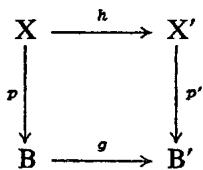
\includegraphics[keepaspectratio]{images/part001_9e08a31f.jpg}}

X (resp. X') be a manifold of class \(C^{r,s}\) over B (resp. B'), and let h be a mapping from X into X'. We say that h is a g-morphism of class \(C^{r,s}\) if the following three conditions are satisfied:

\begin{enumerate}
\def\labelenumi{\alph{enumi})}
\item
  \(p^{\prime}\circ h = g\circ p;\)
\item
  h is continuous;
\item
  for every chart \((\mathrm{V}^{\prime},\psi^{\prime},\mathrm{F}^{\prime})\) of the \(C^{r,s}\) -manifold \(X^{\prime}\) , the map \(pr_{2}\circ\psi^{\prime}\circ h\) of \(V=h^{-1}(V^{\prime})\) to \(F^{\prime}\) is of
\end{enumerate}

class \(\mathbf{C}^{r,s}\) (in the sense of 15.2.4) when one endows the open set V with the structure induced by that of X (15.2.3, (iii)).

When \(\mathbf{B} = \mathbf{B}'\) and \(g = \mathrm{Id}_{\mathbf{B}}\) , we also say that \(h\) is a B-morphism of class \(\mathbf{C}^{r,s}\) .

For a B-morphism of class \(C^{r,s}\) to be a B-isomorphism of class \(C^{r,s}\) , it suffices that it be an isomorphism of class \(C^{1}\) .

Let \(g': B' \to B''\) be a morphism of manifolds of class \(C^r\) and let \(X''\) be a manifold of class \(C^{r,s}\) over \(B''\) . If \(h: X \to X'\) is a \(g\) -morphism of class \(C^{r,s}\) and \(h': X' \to X''\) is a \(g'\) -morphism of class \(C^{r,s}\) , then \(h' \circ h\) is a \((g' \circ g)\) -morphism of class \(C^{r,s}\) .

15.2.6. Let X be a manifold of class \(\mathbf{C}_{\mathbf{R}}^{r,s}\) over B and \(p\) its projection; we assume \(s \neq \omega\) , X is separated, and \(p\) is proper (TG, I, § 10, no. 1). Then, for every \(b \in \mathbf{B}\) there exists an open neighborhood U of \(b\) and a \(\mathbf{C}^{r,s}\) -isomorphism from \(p^{-1}(\mathbf{U})\) onto \(\mathbf{U} \times \mathbf{X}_b\) , where \(\mathbf{X}_b = p^{-1}(b)\) .

15.2.7. Let X be a manifold of class \(C_{K}^{r,s}\) over B, p its projection, and \(\sigma: B \to X\) be a section of class \(C^{r}\) . We call a tubular neighborhood of class \(C_{K}^{r,s}\) of \(\sigma\) a triple (M, N, \(\varphi\) ) where M is a K-vector bundle, with base B and of class \(C^{r}\) , N is an open neighborhood of \(\sigma(\mathbf{B})\) in X, and \(\varphi\) is a B-isomorphism of class \(C_{K}^{r,s}\) from N onto an open subset of M (cf. 15.2.3 (iv)), mapping the section \(\sigma\) to the zero section of M.

Suppose that \(s \geqslant r + 1\) and that the manifold B is paracompact and admits partitions of unity of class \(\mathbf{C}^{r}\) (5.3.6); there then exist tubular neighborhoods of class \(\mathbf{C}_{\mathbb{K}}^{r,s}\) of \(\sigma\) .

\subsection{Varieties of sections and varieties of mappings}

15.3.1 ("Banach space structure on a space of sections"). Let B be a compact differentiable manifold of class \(C^{r}\) ; let M be a vector bundle over K (7.3.4) with base B and of class \(C^{r}\) ; denote by \(M_{r}\) the differentiable manifold of class \(C^{r}\) underlying M, and let \(\mathcal{S}_{\mathrm{M}}^{\tau}(\mathrm{B})\) be the K-vector space of sections of class \(C^{r}\) of M (7.4.1). The topology on \(\mathcal{S}_{\mathrm{M}}^{\tau}(\mathrm{B})\) induced by the topology of \(C^{r}\) -uniform convergence on \(\mathcal{C}^{\tau}(\mathrm{B};\mathrm{M}_{r})\) (12.3.10) makes \(\mathcal{S}_{\mathrm{M}}^{\tau}(\mathrm{B})\) a K-Banach space.

Let \((\mathrm{U}_{i})_{i\in\mathbb{I}}\) be a finite open covering of B and, for every \(i\in I\) , let \(c_{i}=(\mathrm{U}_{i},\varphi_{i},\mathrm{E}_{i})\) be a chart of B and \(t_{i}=(\mathrm{U}_{i},\psi_{i},\mathrm{F}_{i})\) be a K-vector chart of M (8.8.1). Let each of the \(E_{i}\) (resp. \(F_{i}\) ) be equipped with a norm compatible with its structure of Banach space over R (resp. K), and let \((\mathrm{V}_{i})_{i\in\mathbb{I}}\) be a closed covering of B, such that \(V_{i}\subset U_{i}\) for all \(i\in I\) . For \(f\in\mathcal{S}_{\mathrm{M}}^{\tau}(\mathrm{B})\) and \(i\in I\) , denote by \(f_{i}\) the map from \(\varphi_{i}(\mathrm{U}_{i})\) to \(F_{i}\) obtained by composition:

\[
\varphi_ {i} \left(\mathrm{U} _ {i}\right) \xrightarrow {\varphi_ {i} ^ {- 1}} \mathrm{U} _ {i} \xrightarrow {f} \mathrm{M} \left| \mathrm{U} _ {i} \xrightarrow {\psi_ {i}} \mathrm{U} _ {i} \times \mathrm{F} _ {i} \xrightarrow {\operatorname{pr} _ {2}} \mathrm{F} _ {i}. \right.
\]

Set

\[
\| f \| = \operatorname{Sup} _ {i \in I, p \leqslant r, x \in V _ {i}} \| D ^ {p} f _ {i} (\varphi_ {i} (x)) \|.
\]

The map \(f\mapsto\|f\|\) is a norm on \(\mathcal{S}_{\mathrm{M}}^{\tau}(\mathrm{B})\) , which gives \(\mathcal{S}_{\mathrm{M}}^{\tau}(\mathrm{B})\) the structure of a Banach space over K.

If N is an open subset of the space M, the set \(\mathcal{S}^{\tau}(\mathbf{B};\mathbf{N})\) of sections \(f\in\mathcal{S}_{\mathbf{M}}^{\tau}(\mathbf{B})\) such that \(f(\mathbf{B})\subset\mathbf{N}\) is open in \(\mathcal{S}_{\mathbf{M}}^{\tau}(\mathbf{B})\) .

15.3.2. Let B be a compact differentiable manifold of class \(C^{r}\) , and let X be a manifold of class \(C_{K}^{r,s}\) ( \(s \geqslant r + 1\) ) over B. If N is an open subset of X, denote by \(\mathcal{S}^{r}(B; N)\) the set of sections of class \(C^{r}\) of X over B whose image is contained in N. There exists on \(\mathcal{S}^{r}(B; X)\) a K-manifold structure of class \(C^{s-r}\) , and only one, such that, for every section \(\sigma \in \mathcal{S}^{r}(B; X)\) and every tubular neighborhood (M, N, \(\varphi\) ) of class \(C_{K}^{r,s}\) of \(\sigma\) (15.2.7), the triple ( \(\mathcal{S}^{r}(B; N)\) , \(\varphi^{*}\) , \(\mathcal{S}_{M}^{r}(B)\) ), where \(\varphi^{*}\) is the map \(f \mapsto \varphi \circ f\) , is a chart of the K-manifold \(\mathcal{S}^{r}(B; X)\) .

In what follows, we equip \(\mathcal{S}^{r}(\mathbf{B};\mathbf{X})\) of this structure.

15.3.3. Let X be a compact differentiable manifold of class \(C^{r}\) , and let Y be a K-manifold of class \(C^{s}(s \geqslant r + 1)\) . Let \(\mathcal{C}^{r}(X; Y)\) be the set of maps of class \(C^{r}\) from X into Y (in other words, taking values in the manifold of class \(C^{r}\) underlying Y, cf. 5.13.1 and 5.14.2). We equip \(\mathcal{C}^{r}(X; Y)\) with the structure of a K-variety of class \(C^{s-r}\) obtained by identifying it with \(\mathcal{S}^{r}(X; X \times Y)\) , cf. 15.2.3, (ii) and 15.3.2. It is called the variety of mappings of class \(C^{r}\) of X into Y. Its topology is that of \(C^{r}\) -uniform convergence (12.3.10).

Suppose Y is separated; then so is \(\mathcal{C}^{r}(X;Y)\) . Moreover, the set of immersions (resp. embeddings, submersions, surjective submersions, étale morphisms, isomorphisms) of class \(C^{r}\) from X into Y is an open subset of \(\mathcal{C}^{r}(X;Y)\) .

Let \(X'\) be a compact differentiable manifold of class \(C^r\) , \(\varphi: X' \to X\) a morphism of differentiable manifolds of class \(C^r\) and \(\psi: Y \to Y'\) a morphism of K-varieties of class \(C^s\) . The map \(f \mapsto \psi \circ f \circ \varphi\) is a morphism of class \(C^{s-r}\) of \(\mathscr{C}^r(X; Y)\) to \(\mathscr{C}^r(X'; Y')\) .

15.3.4 (“Weakening of structure”). Keep the hypotheses and notations of 15.3.3. Moreover, let \(s' \in \mathbf{N}_{\mathbf{R}}\) satisfy \(r < s' \leqslant s\) and let \(\mathbf{Y}_{s'}\) be the real manifold of class \(\mathbf{C}^{s'}\) underlying \(\mathbf{Y}\) (5.13 and 5.14.2). The structure of real manifold of class \(\mathbf{C}^{s'-r}\) on \(\mathcal{C}^r(\mathbf{X}; \mathbf{Y}_{s'})\) underlies the structure of K-manifold of class \(\mathbf{C}^{s-r}\) on \(\mathcal{C}^r(\mathbf{X}; \mathbf{Y})\) .

15.3.5. Let X and X' be compact differentiable manifolds of class \(C^{r}\) and \(C^{r'}\) , respectively, with \(r' < r\) ; let Y be a K-variety of class \(C^{s}\) , with \(s \geqslant r + 1\) . Let \(t = \operatorname{Inf}(r - r', s - r)\) . The map \((f, g) \mapsto g \circ f\) is a morphism of class \(C^{t}\) from \(\mathcal{C}^{r}(X'; X) \times \mathcal{C}^{r}(X; Y)\) to \(\mathcal{C}^{r'}(X'; Y)\) .

15.3.6 (“Tangent space to \(\mathcal{C}^r (\mathrm{X};\mathrm{Y})\)”). Given the hypotheses of 15.3.3, let \(f\in \mathcal{C}^r (\mathrm{X};\mathrm{Y})\) and let \(\xi\) be a tangent vector at \(f\) to the manifold \(\mathcal{C}^r (\mathrm{X};\mathrm{Y})\) . If \(x\in \mathrm{X}\) , denote by \(\varepsilon_{x}\) the map \(g\mapsto g(x)\) of \(\mathcal{C}^r (\mathrm{X};\mathrm{Y})\) into Y; it is a morphism of class \(\mathbf{C}^{s - r}\) . The image of \(\xi\) under \(\mathrm{T}_f(\varepsilon_x)\) is an element \(\xi_{x}\) of \(\mathrm{T}_{f(x)}(\mathrm{Y})\) ; the map \(x\mapsto \xi_{x}\) is a lifting of class \(\mathbf{C}^r\) of \(f\) in T(Y) (cf. 8.6.1) and it can be identified with a section of class \(\mathbf{C}^r\) of the vector bundle \(f^{*}\mathrm{T}(\mathrm{Y})\) of base X. In this way, one obtains an isomorphism of the tangent space \(\mathrm{T}_f(\mathcal{C}^r (\mathrm{X};\mathrm{Y}))\) onto the Banach space \(\mathcal{S}_{f^{*}\mathrm{T}(\mathrm{Y})}^r (\mathrm{X})\) .

15.3.7 ("Interpretation of \(\mathcal{C}^{p}(\mathrm{X};\mathcal{C}^{q}(\mathrm{Y};\mathrm{Z}))\)"). Let X and Y be compact differentiable manifolds of class \(\mathbf{C}^{p}\) and \(\mathbf{C}^{q}\) respectively ( \(1\leqslant p\leqslant+\infty,1\leqslant q<+\infty\) ), and let Z be a K-variety of class \(\mathbf{C}^{s}\) , with \(s\geqslant p+q\) . Let \(f\colon\mathrm{X}\times\mathrm{Y}\to\mathrm{Z}\) be a continuous map;

for every \(x \in X\) , denote by \(f_x\) the map \(y \mapsto f(x, y)\) from Y to Z. The following two properties are equivalent:

\begin{enumerate}
\def\labelenumi{\alph{enumi})}
\item
  For any charts \(c = (\mathrm{U}, \varphi, \mathrm{E})\) of \(\mathbf{X}\) , \(d = (\mathrm{V}, \psi, \mathrm{F})\) of \(\mathbf{Y}\) and \(e = (\mathrm{W}, \theta, \mathrm{G})\) of \(\mathbf{Z}\) such that \(f(\mathrm{U} \times \mathrm{V}) \subset \mathrm{W}\) , the partial derivatives \(\mathrm{D}_{\mathbb{E}}^{p'} \mathrm{D}_{\mathbb{F}}^{q'} f'\) of the expression \(f'\) of \(f\) in the charts \(c \times d\) and \(e\) (5.3.2) exist and are continuous for \(p' \leqslant p\) and \(q' \leqslant q\) .
\item
  For every \(x \in X\) , the map \(f_{x}\) is of class \(C^{q}\) and the map \(x \mapsto f_{x}\) is a morphism of class \(C^{p}\) from X into the variety \(\mathcal{C}^{q}(Y; Z)\) .
\end{enumerate}

\pandocbounded{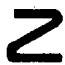
\includegraphics[keepaspectratio]{images/part001_50717dae.jpg}}

15.3.8. Let Y be a compact K-variety of class \(C^{s}\) , with \(s \geqslant r + 1\) , and let \(\text{Diff}^{r}(Y)\) be the group of automorphisms of class \(C^{r}\) of the real manifold \(Y_{r}\) of class \(C^{r}\) underlying Y. The set \(\text{Diff}^{r}(Y)\) is open in \(\mathcal{C}^{r}(Y; Y) = \mathcal{C}^{r}(Y_{r}; Y)\) ; we endow it with the structure of a K-variety of class \(C^{s-r}\) induced by that of \(\mathcal{C}^{r}(Y; Y)\) . The composition law \((f, g) \mapsto g \circ f\) makes \(\text{Diff}^{r}(Y)\) a topological group. On the other hand, the manifold structure of class \(C^{s-r}\) is not in general compatible with the group structure of \(\text{Diff}^{r}(Y)\) . For \(f \in \text{Diff}^{r}(Y)\) , the map \(g \mapsto g \circ f\) of \(\text{Diff}^{r}(Y)\) into itself is of class \(C^{s-r}\) , but the map \(g \mapsto f \circ g\) is not in general of class \(C^{1}\) . In particular, \(\text{Diff}^{r}(Y)\) is not in general a Lie group.\footnote{Suppose that \(s = \infty\). Let \(\text{Diff}^{\infty}(Y)\) be the group of automorphisms of class \(C^{\infty}\) of Y; equip it with the coarsest topology making the canonical injections \(\text{Diff}^{\infty}(Y) \to \text{Diff}^{r}(Y)\), for every integer \(r \geqslant 1\), continuous. On the other hand, let \(\text{Diff}^{0}(Y)\) be the group of homeomorphisms of Y, endowed with the topology of uniform convergence (TG, X, § 3, no. 5, Proposition 11). If \(\dim Y \geqslant 1\), it is impossible to find a Lie group G and continuous homomorphisms from \(\text{Diff}^{\infty}(Y)\) to G and from G to \(\text{Diff}^{0}(Y)\) whose composite is the canonical injection (cf. LIE, III, § 4, Exercise 7).}

\specialchapter{INDEX OF NOTATIONS}

\(N_{K}\) : Notations and conventions T(X): 8.1.1 \(\zeta_{c}\) : 8.1.1 T(f): 8.1.2 T(X/Y): 8.1.3 \((\partial/\partial u^{i})\) : 8.1.5 T'(X): 8.2.2 df: 8.2.2 \(\langle\xi, df\rangle\) , D \(_{\xi}(f)\) , \(\xi(f)\) : 8.2.3 \(\varphi^{*}\eta\) : 8.2.6 \(\varphi^{*}\omega\) : 8.2.7 and 8.3.1 \(^{k}\Omega^{p}(U; E)\) : 8.3.1 \(\omega|Y\) : 8.3.1 \(\omega\wedge\omega'\) : 8.3.2 \(i(\xi,\omega)\) , \(i(\xi)\omega\) , \(i(\xi).\omega\) : 8.3.2 \(d\omega\) : 8.3.5 GL(E): 8.4.1 \(\theta_{\xi}.f\) : 8.4.2 \([\xi,\eta]\) : 8.5.1 \(i(\psi,\omega)\) , \(i(\psi)\omega\) , \(i(\psi).\omega\) : 8.6.2 F ⊗ C: 8.8.2 T'(X), T''(X): 8.8.3 Alt \(^{p,q}\) (T(X); F): 8.8.4 \(\omega_{p,q}\) : 8.8.4 \(d'\omega\) , \(d''\omega\) : 8.8.5 \(\partial/\partial z^{k}\) , \(\partial/\partial\bar{z}^{k}\) : 8.8.10 \(dz^{\Delta}\) , \(d\bar{z}^{\Delta}\) : 8.8.10 \(\alpha_{+}\) , \(\alpha_{-}\) , \(\Omega\) : 9.1.4 \(\rho\) , \(\Delta\) : 9.1.5 \(X_{p}\) : 9.2.1 T(X,Y): 9.2.8 F': 9.3.7 \(\xi^{p}\) : 9.4.1 \(\Lambda_{p}(x,y)\) : 9.4.2

\(\mu^{\otimes n}, \mu_{\mathrm{U}}^{\otimes n}: 10.1\)

mod(a): 10.1

Jac(f): 10.1.1

mod(\(\omega\))\(_{\mu}\), \(|\omega|\): 10.1.6

\(\xi'\xi''\), \(\xi''\xi': 10.2.1\)

Or(E): 10.2.1

\(\mathrm{Or}_{\mathrm{M}}\): 10.2.2

\(\lambda_{\mathrm{M}} = (\mathrm{Or}_{\mathrm{M}}, \{\pm 1\}, \mathrm{X}, \pi)\): 10.2.2

\(\tilde{\mathbf{X}}\): 10.2.4

\(\xi_1 \otimes \xi_2: 10.2.6\) \(\tilde{\mathbf{R}}_{\mathrm{M}}\): 10.3.1

\(\tilde{\mathbf{R}}_{\mathbf{X}}\): 10.4.1

\(\alpha(\omega), \int_{\mathbf{X}} g \cdot \omega, \int_{\mathbf{A}} \omega: 10.4.3\) \(\omega|_{\mathrm{Y}}: 10.4.3\) \(\partial A: 11.1.2\) and 11.3.2

\(\mathrm{T}_a^+(\mathrm{A}), \mathrm{T}_a^-(\mathrm{A}): 11.1.4\) \(\omega|_{\partial A}: 11.2.2\) \(u \perp (t_1, \ldots, t_p): 11.4.1\) \(\tilde{\mathbf{R}}_n: 11.4.2\) \(\omega \perp (t_1, \ldots, t_p): 11.4.5\) \(\int_{\pi|_{\mathrm{A}}} \omega, \int_{\pi} \omega: 11.4.6\) \(j_x^k(f): 12.1.2\) \(s(j), b(j): 12.1.2\) \(\mathrm{J}^k(\mathrm{X}, \mathrm{Y}), \mathrm{J}_x^k(\mathrm{X}, \mathrm{Y}), \mathrm{J}^k(\mathrm{X}, \mathrm{Y})_y, \mathrm{J}_x^k(\mathrm{X}, \mathrm{Y})_y: 12.1.2\) \(j' \circ j: 12.1.4\) \(r^{k, k'}(j): 12.1.5\) \(j_x^\infty(f), j_x^\omega(f): 12.1.6\) \(\mathrm{P}_m(\mathrm{E}; \mathrm{F}): 12.2\) \(\Delta^m f(a), \Delta_a^m(f), \Delta_a^m(j): 12.2.1\) \(\mathrm{Q}^k(\mathrm{E}, \mathrm{F}): 12.2.2\) \(\mathrm{T}(j): 12.3.4\) \(j^k(f): 12.3.7\) \(\mathrm{J}^k(f, g): 12.3.9\) \(\mathrm{GL}^k(\mathrm{E}): 12.4.2\) \(\mathrm{R}^k(\mathrm{E}, \mathrm{X}): 12.4.3\) \(\mathrm{P}_x^k(\pi), \mathrm{P}^k(\pi): 12.5.1\) \(\mathrm{P}^k(g): 12.5.3\) \(\mathrm{P}^k(\mathrm{E}): 12.6.1\) \(\mathrm{P}^k(\mathrm{X}): 12.6.2\) \(\mathrm{P}^k(u): 12.6.3\) \(\tau_m(\mathcal{V}), \tau_m(f), \mathrm{P}_m(\mathrm{E}; \mathrm{F}): 12.6.7\) \(\mathrm{TS}^n(\mathrm{E}), \mathrm{TS}(\mathrm{E}), \mathrm{TS}^{(r)}(\mathrm{E}), \mathrm{TS}^{(r)+}(\mathrm{E}): 13.1.1\) \(\gamma_n(x): 13.1.1\) \(\langle f, t\rangle\): 13.1.2, 13.1.3, 13.2.2, 13.6.1

\(\varphi_{*}(t)\) : 13.1.4 \(\mathrm{T}_x^{(r)}(\mathrm{X}), \mathrm{T}_x^{(k)}(\mathrm{X}), \mathrm{T}_x^{(k)+}(\mathrm{X})\) : 13.2.1 \(\varepsilon_x\) : 13.2.1 \(\langle j, t \rangle\) : 13.2.2 \(\mathrm{T}_x^{(r)}(\varphi), \varphi_*\) : 13.2.3, 13.6.1 \(\mathrm{T}^{(k)}(\mathrm{X}), \mathrm{T}^{(k)+}(\mathrm{X})\) : 13.2.5 \((\Delta_{\xi}^{\alpha})_a\) : 13.2.6 \(\mathrm{gr}_k \mathrm{T}_x^{(r)}(\mathrm{X}), \mathrm{gr} \mathrm{T}_x^{(r)}(\mathrm{X})\) : 13.3.1 \(i, i_x, i_X, i_{X,x}\) : 13.3.1 \(i_k\) : 13.3.1 \(\mathrm{gr}(\varphi_x)\) : 13.3.5 \(t_1 \times t_2, t_1 \otimes t_2\) : 13.4.1 \(\mathrm{T}_x^{(n)}(\mathrm{X}_1, \mathrm{X}_2)\) : 13.4.5 \(\Delta_*\) , \(c\) : 13.5.1 \(\mathcal{T}^{(k)}(\mathrm{X})\) : 13.6.1 \(\mathrm{D}^k (\mathrm{E}, \mathrm{F})\) : 14.1.1 \(\mathcal{D}_{\mathrm{U}}^{k,h}(\mathrm{E}, \mathrm{F})\) : 14.1.1 \(\operatorname{ad}(f)\theta\) : 14.1.4 \(\Delta^\alpha\) : 14.1.6 \(\mathrm{D}_{\mathbf{C}}^{k}(\mathrm{E}, \mathrm{F})\) : 14.1.7 \(\mathrm{D}'' \circ \mathrm{D}'\) : 14.1.8 \([\mathrm{D}' , \mathrm{D}'']\) : 14.1.8 \(\mathrm{S}^k (\mathrm{E}, \mathrm{F})\) : 14.2.1 \(\sigma_k (\mathrm{D})\) : 14.2.1 \(\mathrm{Sym}^k (\mathrm{M}; \mathrm{N})\) : 14.2.2 \(\Omega, \tilde{\mathbf{M}}\) : 14.3.1 \(^t\mathbf{D}\) : 14.3.2 \(\Omega_1, \mathbf{G}\) : 14.3.4 \(\Omega^p\) : 14.4.2 \(\operatorname{grad}(f)\) : 14.4.3 \(\mathbf{C}_{\mathbf{R}}^{r,s}\) : 15.1.1 \(\mathbf{C}_{\mathbf{K}}^{r,\omega}\) : 15.1.2 \(\mathbf{C}^{r,s}\) : 15.1.1, 15.1.2, 15.1.6, 15.2.1 \(\mathcal{S}_{\mathbf{M}}^r (\mathbf{B})\) : 15.3.1 \(\mathcal{S}^r (\mathbf{B}; \mathbf{N})\) : 15.3.1 and 15.3.2 \(\mathcal{C}^r (\mathbf{X}; \mathbf{Y})\) : 15.3.3\\
Diff'(Y): 15.3.8

\specialchapter{TERMINOLOGICAL INDEX}

adapted to a piece (chart): 11.1.2 weakening of the structure of a vector bundle: 8.7.1 integral arc, maximal integral arc: 9.1.3 C-vector atlas, complex vector atlas: 8.8.1 boundary of a closed half-space: 11.1.1 boundary of a piece: 11.1.2 boundary (manifold with): 11.1. Note (1) B-morphism of class \(\mathbf{C}^{r,s}\) : 15.2.5 target of a jet: 12.1.2 chart of a manifold of class \(\mathbf{C}^{r,s}\) over B: 15.2.1 C-vector chart, complex vector chart: 8.8.1 chart over B: 15.2.1 Cauchy (formula of): 11.2.5 field of point distributions: 13.2.5 field of point distributions of class \(\mathbf{C}^s\) : 13.2.5 vector field: 8.2.1 complex vector field: 8.8.2 covector field: 8.2.2 initial field: 8.4.5 class \(\mathbf{C}^0\) (manifold of, morphism of): Notations and Conventions class \(\mathbf{C}^{r,s}\) (function of): 15.1.1 and 15.1.2 class \(\mathbf{C}^{r,s}\) (map of): 15.1.6 and 15.2.4. class \(\mathbf{C}^{r,s}\) (g-morphism of): 15.1.6 and 15.2.5 class \(\mathbf{C}^{r,s}\) over B (manifold of): 15.2.1 canonical class of measures: 10.1.4 class of a differential operator: 14.1.1 complexification of a vector bundle: 8.8.2 component of type \((p,q)\) : 8.8.4 composite of two jets: 12.1.4 composite of two differential operators: 14.1.8 conjugate (section): 8.8.2 contact of order ≥k: 12.1.1 contact of infinite order: 12.1.6 contravariant (functor): 8.2.7

coproduct of a point distribution: 13.5.1 integral curve: 9.1.1 and 9.1.7 bracket: 8.5.1 \(\mathbf{C}^{r,s}\)-compatible (charts over B): 15.2.1 \(\mathbf{C}^{r,s}\)-atlas: 15.2.1 C-vector (bundle, chart, atlas): 8.8.1 closed half-space: 11.1.1 differential of a function: 8.2.2 exterior differential: 8.3.5 and 10.3.4 distribution with finite support: 13.6.1, 13.6.2 complex distribution with finite support: 13.6.2 point distribution: 13.2.1 point distribution of order ≤k: 13.2.1 distribution without constant term: 13.2.1 leaf: 9.2.2 connected leaf: 9.2.2 foliation: 9.2.2 discrete, coarse foliation: 9.2.4 induced foliation, inverse image: 9.2.5 foliating (chart): 9.2.7 foliated (manifold): 9.2.2 cotangent bundle: 8.2.2 C-vector bundle: 8.8.1 normal bundle: 8.1.3 tangent bundle: 8.1.1 tangent bundle to the fibers: 8.1.3 relative tangent bundle: 8.1.3 transverse bundle: 8.1.3 complex vector bundle: 8.8.1 real vector bundle: 8.8.1 integral flow: 9.1.2 differential form: 8.3.1 alternating differential form: 8.3.1 differential form of maximum degree: 10.1.5 holomorphic (differential form, vector field): 8.8.9 horizontal (section): 9.2.10 odd (differential form): 10.4.1 induced (differential form): 8.3.1 and 11.2.2 integrable (vector subbundle): 9.3.2 and 9.4.4 integrable (differential form): 10.4.3 locally integrable (differential form): 10.4.3 integral (foliation): 9.3.2 integral (submanifold): 9.3.1 integral (of an equation in total differentials): 9.3.7 integral of a vector subbundle: 9.3.1

integration along the fibers: 11.4.6 lifetime interval: 9.1.3 Jacobian: 10.1.1 jet: 12.1.2 jet of infinite order: 12.1.6 jet of a section: 12.5.1 modulus of a differential form: 10.1.6 locally integrable modulus: 10.1.5 M-twisted (differential forms): 10.3.3 M-twisted (bundle of scalars): 10.3.1 negligible (locally negligible set): 10.1.3 Green operator: 14.3.4 complex differential operator: 14.1.7 differential operator of bounded order: 14.1.1 differential operator of type E → F, of order ≤k: 14.1.1 multidifferential operator: 14.1.11 order of a differential operator: 14.1.1 orientable (vector bundle): 10.2.3 orientable (manifold): 10.2.4 orientation defined by a complex structure: 10.2.7 orientation of a manifold: 10.2.4 orientation of a vector bundle: 10.2.3 orientation of a morphism: 10.2.5 orientations (space of): 10.2.2 even (differential form): 10.4.1 piece: 11.1.2 polyhedral (part): 11.3.1 locally polyhedral (part): 11.3.1 homogeneous polynomial (map): 13.1.2 almost complex (structure): 8.8.3 product of orientations: 10.2.6 exterior product: 8.3.2 interior product: 8.3.2 and 8.6.2 projection of a manifold of class \(\mathbf{C}^{r,s}\) over B: 15.2.1 regular (point, boundary): 11.3.2 lifting: 8.6.1 inward (vector, strictly inward vector): 11.1.4 frame of order k: 12.4.3 tangent frame: 8.1.5 Sard (theorems of): 10.1.3 scalar (differential operator): 14.1.6 scalar (multidifferential operator): 14.1.11 section of a fibration: Notations and conventions S-orientation of an S-morphism: 11.4.3 outward (vector, strictly outward vector): 11.1.4

source of a jet: 12.1.2

Stokes (formula of): 11.2.3 and 11.3.4

support of a differential form: 10.4.3

symbol of a differential operator: 14.2.1

tangent (bundle): 8.1.1

tangent to a foliation (subbundle): 9.2.8

constant term of a point distribution: 13.2.1

twisted (differential forms): 10.4.1

topology of uniform \(C^{k}\)-convergence: 12.3.10

twisted (scalar bundle): 10.4.1

transpose of a differential operator: 14.3.2

type \((p,q)\) (differential form of): 8.8.4

manifold of mappings of class \(\mathbf{C}^r\) : 15.3.3

velocity: 9.1.1

tubular neighborhood: 15.2.7

π-twisted (differential form): 11.4.2

\(\varphi\)-related: 8.2.6


